\documentclass[conference]{IEEEtran}
\IEEEoverridecommandlockouts
% The preceding line is only needed to identify funding in the first footnote. If that is unneeded, please comment it out.
\usepackage{cite}
\usepackage{amsmath,amssymb,amsfonts}
\usepackage{algorithmic}
\usepackage{graphicx}
\usepackage{textcomp}
\usepackage{xcolor}
\usepackage{hyperref} %url
\usepackage{booktabs}
\usepackage{tikz}
\usepackage{pgfplots}
\usepackage{pgfplotstable}
\usepackage{filecontents}
\usetikzlibrary{snakes,arrows,shapes,backgrounds, positioning,fit,calc}
\usetikzlibrary{decorations.text}
\usetikzlibrary{decorations.pathmorphing}





% Farbpalette A
\definecolor{blau_1a}{RGB}{93,133,195}
\definecolor{blau_2a}{RGB}{0,156,218}
\definecolor{gruen_3a}{RGB}{80,182,149}
\definecolor{gruen_4a}{RGB}{175,204,80}
\definecolor{gruen_5a}{RGB}{221,223,72}
\definecolor{orange_6a}{RGB}{255,224,92}
\definecolor{orange_7a}{RGB}{248,186,60}
\definecolor{rot_8a}{RGB}{238,122,52}
\definecolor{rot_9a}{RGB}{233,80,62}
\definecolor{lila_10a}{RGB}{201,48,142}
\definecolor{lila_11a}{RGB}{128,69,151}

% Farbpalette B
\definecolor{blau_1b}{RGB}{0,90,169}
\definecolor{blau_2b}{RGB}{0,131,204}
\definecolor{gruen_3b}{RGB}{0,157,129}
\definecolor{gruen_4b}{RGB}{153,192,0}
\definecolor{gruen_5b}{RGB}{201,212,0}
\definecolor{orange_6b}{RGB}{253,202,0}
\definecolor{orange_7b}{RGB}{245,163,0}
\definecolor{rot_8b}{RGB}{236,101,0}
\definecolor{rot_9b}{RGB}{230,0,26}
\definecolor{lila_10b}{RGB}{166,0,132}
\definecolor{lila_11b}{RGB}{114,16,133}

\colorlet{mygreen}{green!80!black}
\colorlet{myblue}{blue!80!black}
\colorlet{myred}{red!80!black}

\ifCLASSOPTIONcompsoc
\usepackage[caption=false,font=normalsize,labelfont=sf,textfont=sf]{subfig}
\else
\usepackage[caption=false,font=footnotesize]{subfig}
\fi

\usetikzlibrary{external}
\tikzexternalize[prefix=tikz/]
\tikzexternalize[prefix=tikz/,shell escape=-enable-write18]
\tikzset{external/system call= {pdflatex %-save-size=80000 
%                           -pool-size=10000000 
 %                          -extra-mem-top=50000000 
 %                          -extra-mem-bot=10000000 
  %                         -main-memory=90000000 
                           \tikzexternalcheckshellescape 
                           -halt-on-error 
                           -interaction=nonstopmode
                           -jobname "\image" "\texsource"}} 
                           
                           
                              
\begin{document}

\title{CM3: Convolutional-Max and Mathematical Morphology to Image Segmentation
\thanks{The authors are grateful to FAPEMIG (PPM 00006-16), CNPq (Universal 421521/2016-3 and PQ 307062/2016-3), CAPES (MAXIMUM STIC-AmSUD 048/14) and PUC Minas for the financial support to this work.}
}

\author{\IEEEauthorblockN{Felipe Augusto Lima Reis, Raquel Almeida, Silvio Jamil F. Guimar\~aes, Zenilton K. G. do Patroc\'inio Jr}
\IEEEauthorblockA{\textit{Audio-Visual Information Processing Laboratory (VIPLAB)} \\
\textit{Pontifical Catholic University of Minas Gerais (PUC Minas)}\\
Belo Horizonte, Minas Gerais, Brazil \\
\{falreis, raquel.almeida.685026\}@sga.pucminas.br, \{sjamil, zenilton\}@pucminas.br}
}

\maketitle

\begin{abstract}
Image segmentation refers to the partition of an image into a set of regions representing meaningful areas and it is an active topic of research.  In this work it is proposed to explore the learned model in a deep architecture, presenting a strategy to combine side outputs extracted at different layers of the network. It is also proposed to study the impact of the amount of side outputs extracted and the impact of a post-processing strategy using mathematical morphology. Experiments demonstrated that proposed approach is viable and  achieve results comparable or superior to the state-of-the-art for the public available KITTI Road/Lane Dataset for image segmentation.
\end{abstract}

%\begin{IEEEkeywords}
%component, formatting, style, styling, insert
%\end{IEEEkeywords}

\section{Introduction}
\label{sec:intro}

Image segmentation refers to the partition of an image into a set of regions representing  meaningful areas, and it is considered as a challenging semantic task, aiming to determine and group uniform regions for analysis. According to~\cite{DOMINGUEZ}, to create an adequate segmented image it is necessary that the output presents some fundamental characteristics, such as: (i) region uniformity and homogeneity in  its features, such as gray level, color or texture; (ii) region continuity, without holes; (iii) significant difference to adjacency regions; and (iv) spatial accuracy with smooth boundaries and without raggedness. Image segmentation is still an active topic of research and, usually, it could be divided in two stages~\cite{guigues06}: (i) low-level analysis, which evaluate the pixel characteristics, neighboring relation and it is ideally uncommitted in terms of position, orientation, size and contrast; and (ii) high-level analysis, which maps the low-level characteristics to fulfill the task.  

Recently, deep learning approaches have drastically changed the computational paradigm for visual tasks. The main advantage of deep learning algorithms is that it does not require an engineered model to operate, meaning that they are capable of learning not only the features to represent the data but also the models to describe it~\cite{goodfellow16}. Facing with this new paradigm, researches initially replaced  hand-craft features in the low-level analysis by the features learned in deep models~\cite{farabet2013,simonyan2014,lee2015}, which mostly achieved the desirable results. More recently, there are many proposals which explore the learned model for the high-level analysis in order to create maps from the outputs of different layers in a deep learning network~\cite{xie2017,cheng2016,maninis2017,liu2017}. 

%% IT IS IMPORTANT TO DEFINE CONCEPT...
One challenge on the latter strategy is how to combine the output from distinct layers, considering that they are presented with different sizes and could represent different concepts. In this work, we propose some strategies to combine the outputs from different layers by using simple merging functions in order to explore useful behavior in the learning process. We also study of the amount of combined side outputs which are necessary to create a viable region proposition for the task of road image segmentation. Moreover, we propose the use of a post-processing filtering based on mathematical morphology idempotent functions~\cite{najman13} in order to remove some underisable small segments.
%, more specifically,  an area opening mathematical morphology idempotent functions~\cite{najman13} to better cope with the fundamental characteristics of an ideal segmented image.  

The remainder of this work is organized as follows. In Section~\ref{sec:related}, some related works are described in order to characterize the hierarchy of concepts in deep models. In Section~\ref{sec:method}, the proposed method as well the reasoning and strategies are presented. In Section~\ref{sec:experiments}, a quantitative and qualitative assessment are done. And, finally, in Section~\ref{sec:conclusion}, some conclusions are drawn.



\section{Related work}
\label{sec:related}




Deep learning approaches were initially described as black-box methods, meaning that not much were known about the reasoning and decisions of the created models. Much exertion have been applied to investigate the networks operation, whether by methodical experimentation~\cite{ilin17,kuo16,eigen14,zhang17} or visualization methods~\cite{simonyan13,zeiler14}. Those efforts provided more clarity of the deep models and characterized the learned features as complex concepts build from simpler ones. Also it demonstrate the learning progression from detailed to coarser representations as the scale and resolutions reduce through the network.  When applied for object recognition task for instance, the raw pixel on the input layer is learned as segments and parts until the composition of an object concept on posterior layers, while the input scale reduces to a single feature vector on the output.  

The knowledge of the concept abstraction and learning progression allowed new research endeavors to explore  them in high-level tasks. For instance, three main architectures standout in recent years, namely: (i) Holistically-nested Edge Detection~(HED)~\cite{xie2015}; (ii) Convolutional Oriented Boundaries~(COB)~\cite{maninis2017}; and (iii) Rich Convolutional Features~(RCF)~\cite{liu2017}. These architectures explicit explore the models of a traditional deep network to perform a certain high-level task, in which all extract side-outputs of the network and each present a different strategy to combine them . 

The HED network create a side-output layer at each stage of the VGG16 network~\cite{simonyan2014} as boundary maps. In HED, each side-output is associated with a classifier in a deeply supervised scheme~\cite{lee2015} for the task of edge detection. This association insert the fusion process in the network, attributing weights for each side-output that will be learned individually and determine its contribution on the final evaluation. The evaluation is performed by a cost-sensitive function to balance the bias towards non-edge pixels. The HED network significantly improved the performance in multiple datasets and the extended version~\cite{xie2017} also applied the network for the segmentation task. 

The authors in~\cite{cheng2016} use the edge maps created by the HED network alongside with other features such as brightness, colors, gradient and variance to describe images. The goal of their proposal was to create an efficient framework to be used as real-time segmentation system, focused on a fusion strategy to update region features.


In the COB network, the authors also create edge maps from side activations, differing mainly from HED by the attribution to candidate contours orientation information and weights representing the contour strength. The contour orientations are estimated by approximation to known polygon segments and the segments weights are computed based on the candidate contour neighboring region used as a confidence measure. To combine the side outputs it is used a non-linear function to regress both the segment weights and the orientation maps, creating region hierarchical trees by thresholding the contour strength. The network perform well in multiple tasks such object proposal, object detection, semantic contour and segmentation.


Finally, the RCF network, that not only create multiple side-outputs, but also uses multiple scales of the images in the input layer. Differently from the HED network, RCF extract one side-output at each convolutional layer of VGG, arguing that  this could create more detailed representations and improve the network accuracy. The merging process is performed by a series of operations, comprising grouping by convolutions, element-wise sums, up-samplings, local loss functions and concatenation.  



%Regarding the fusion methods, in the aforementioned related strategies, the HED fusion process is also inserted in the network, in which it is attributed weights for each side output that will be learned individually and determine its contribution on the final evaluation. The RCF instead, adopted a $1\times1$ convolution after each output, followed by a element-wise sum, an up-sampling and a loss function. The values are then concatenated and pass through a $1\times1$ convolution for the final evaluation. Finally, the COB network evaluates the The side outputs and the contour orientation maps are evaluated individually creating multiple proposal that could be thresholded based on the confidence value at later stage.  



%\begin{figure*}[!ht]
%\begin{center}
%\begin{tabular}{l}
%(1a) Side outputs extracted at each stage\\
%\resizebox{\textwidth}{!}{%
\begin{tikzpicture}[
std/.style={
  draw,
  text width=1.5cm,
  align=center,
  font=\strut\sffamily
  },
rnd/.style={
  draw=#1,
  rounded corners=8pt,
  line width=1pt,
  align=center,
  text width=2cm,
  minimum height=1cm,
  font=\strut\sffamily
  },
vac/.style={
  text width=2.5cm,
  align=center,
  font=\strut\sffamily
  },
ar/.style={
  ->,
  >=latex
  },
node distance=0.5cm and .5cm    
]



%The nodes for the left
\node[rnd] (inp)
  {Input layer};
\node[rnd=gruen_4b,right=of inp] (conv1)
  {Convolution};  
\node[rnd=gruen_4b,right=of conv1] (conv2)
  {Convolution};  
\node[draw,dashed,gruen_4b,inner sep=8pt,fit={(conv1) (conv2)}]
  (fit) {};
\node[rnd,right=1cm of conv2] (pool1)
  {Pooling};
\node[vac,left=-1cm of pool1, yshift=-1.5cm] (h1)
  {$\mathcal{H}_1$}; 
\node[vac,gruen_4b,left=-1cm of conv2, yshift=1cm] (s1)
  {Stage 1};   
\node[vac,right=-1cm of pool1] (p)
  {$\mathbf{\cdots}$}; 
  
\node[rnd=gruen_4b,right=-.7cm of p] (conv3)
  {Convolution};  
\node[rnd=gruen_4b,right=of conv3] (conv4)
  {Convolution};  
\node[rnd=gruen_4b,right=of conv4] (conv5)
  {Convolution};    
\node[draw,dashed,gruen_4b,inner sep=8pt,fit={(conv3) (conv5)}]
  (fit2) {};
\node[rnd,right=1cm of conv5] (pool2)
  {Pooling};
\node[vac,left=-1cm of pool2, yshift=-1.5cm] (h2)
  {$\mathcal{H}_n$};
  \node[vac,gruen_4b,left=-3cm of conv4, yshift=1cm] (s2)
  {Stage $N$};   
\node[vac,right=-1cm of pool2] (p2)
  {$\mathbf{\cdots}$};   

%Aux  
\coordinate (aux1) at ( $ (conv2.east|-conv2.west)!0.6!(pool1.west) $ );
\coordinate (aux2) at ( $ (conv5.east|-conv5.west)!0.6!(pool2.west) $ );

\draw[ar]  (inp) -- (conv1); 
\draw[ar]  (conv1) -- (conv2); 
\draw[ar]  (conv2) -- (pool1); 
\draw[ar,left=-1cm of pool1, yshift=-1.5cm]  (aux1) -- (h1); 
\draw[ar]  (conv3) -- (conv4);
\draw[ar]  (conv4) -- (conv5); 
\draw[ar]  (conv5) -- (pool2); 
\draw[ar,left=-1cm of pool2, yshift=-1.5cm]  (aux2) -- (h2); 
\end{tikzpicture}%
}\\
%(1b) Side outputs extracted at each convolutional layer\\
%\resizebox{\textwidth}{!}{%
\begin{tikzpicture}[
std/.style={
  draw,
  text width=1.5cm,
  align=center,
  font=\strut\sffamily
  },
rnd/.style={
  draw=#1,
  rounded corners=8pt,
  line width=1pt,
  align=center,
  text width=2cm,
  minimum height=1cm,
  font=\strut\sffamily
  },
vac/.style={
  text width=2.5cm,
  align=center,
  font=\strut\sffamily
  },
ar/.style={
  ->,
  >=latex
  },
node distance=0.5cm and .5cm    
]



%The nodes for the left
\node[rnd] (inp)
  {Input layer};
\node[rnd=lila_10b,right=of inp] (conv1)
  {Convolution};  
\node[rnd=lila_10b,right=of conv1] (conv2)
  {Convolution};  
\node[rnd,right=1cm of conv2] (pool1)
  {Pooling};
\node[vac,right=-1cm of pool1] (p)
  {$\mathbf{\cdots}$}; 
  
\node[rnd=lila_10b,right=-.7cm of p] (conv3)
  {Convolution};  
\node[rnd=lila_10b,right=of conv3] (conv4)
  {Convolution};  
\node[rnd=lila_10b,right=of conv4] (conv5)
  {Convolution};    
\node[rnd,right=1cm of conv5] (pool2)
  {Pooling};
\node[vac,right=-1cm of pool2] (p2)
  {$\mathbf{\cdots}$};   

\node[vac,left=-1cm of conv2, yshift=-1.5cm] (h1)
  {$\mathcal{H}_1$};
\node[vac,left=-1cm of pool1, yshift=-1.5cm] (h2)
  {$\mathcal{H}_2$};    
\node[vac,left=-1cm of conv4, yshift=-1.5cm] (h3)
  {$\mathcal{H}_{n-2}$};
\node[vac,left=-1cm of conv5, yshift=-1.5cm] (h4)
  {$\mathcal{H}_{n-1}$};
\node[vac,left=-1cm of pool2, yshift=-1.5cm] (h5)
  {$\mathcal{H}_n$};


%Aux  
\coordinate (aux1) at ( $ (conv1.east|-conv1.west)!0.3!(conv2.west) $ );
\coordinate (aux2) at ( $ (conv2.east|-conv2.west)!0.6!(pool1.west) $ );
\coordinate (aux3) at ( $ (conv3.east|-conv3.west)!0.3!(conv4.west) $ );
\coordinate (aux4) at ( $ (conv4.east|-conv4.west)!0.3!(conv5.west) $ );
\coordinate (aux5) at ( $ (conv5.east|-conv5.west)!0.6!(pool2.west) $ );

\draw[ar]  (inp) -- (conv1); 
\draw[ar]  (conv1) -- (conv2); 
\draw[ar]  (conv2) -- (pool1); 
\draw[ar]  (conv3) -- (conv4);
\draw[ar]  (conv4) -- (conv5); 
\draw[ar]  (conv5) -- (pool2); 

\draw[ar,left=-1cm of pool1, yshift=-1.5cm]  (aux1) -- (h1);
\draw[ar,left=-1cm of pool2, yshift=-1.5cm]  (aux2) -- (h2); 
\draw[ar,left=-1cm of pool2, yshift=-1.5cm]  (aux3) -- (h3);
\draw[ar,left=-1cm of pool2, yshift=-1.5cm]  (aux4) -- (h4);
\draw[ar,left=-1cm of pool2, yshift=-1.5cm]  (aux5) -- (h5);   

\end{tikzpicture}%
}\\
%\end{tabular}%
%\caption{Illustration for  the proposed side outputs extraction one following the HED model~(a) at each stage of the VGG network and the other following RCF model~(b) at each convolutional layer}
%\end{center}
%\label{fig:methods}
%\end{figure*}
%\section{Convolutional side-outputs for image segmentation}
\section{Side-outputs merging strategies and mathematical morphology post-processing}
\label{sec:method}

\begin{figure*}[!t]
\centering
\subfloat[Stage Layer Outputs (SLO)]{\resizebox{\textwidth}{!}{%
\begin{tikzpicture}[
std/.style={
  draw,
  text width=1.5cm,
  align=center,
  font=\strut\sffamily
  },
rnd/.style={
  draw=#1,
  rounded corners=8pt,
  line width=1pt,
  align=center,
  text width=2cm,
  minimum height=1cm,
  font=\strut\sffamily
  },
vac/.style={
  text width=2.5cm,
  align=center,
  font=\strut\sffamily
  },
ar/.style={
  ->,
  >=latex
  },
node distance=0.5cm and .5cm    
]



%The nodes for the left
\node[rnd] (inp)
  {Input layer};
\node[rnd=gruen_4b,right=of inp] (conv1)
  {Convolution};  
\node[rnd=gruen_4b,right=of conv1] (conv2)
  {Convolution};  
\node[draw,dashed,gruen_4b,inner sep=8pt,fit={(conv1) (conv2)}]
  (fit) {};
\node[rnd,right=1cm of conv2] (pool1)
  {Pooling};
\node[vac,left=-1cm of pool1, yshift=-1.5cm] (h1)
  {$\mathcal{H}_1$}; 
\node[vac,gruen_4b,left=-1cm of conv2, yshift=1cm] (s1)
  {Stage 1};   
\node[vac,right=-1cm of pool1] (p)
  {$\mathbf{\cdots}$}; 
  
\node[rnd=gruen_4b,right=-.7cm of p] (conv3)
  {Convolution};  
\node[rnd=gruen_4b,right=of conv3] (conv4)
  {Convolution};  
\node[rnd=gruen_4b,right=of conv4] (conv5)
  {Convolution};    
\node[draw,dashed,gruen_4b,inner sep=8pt,fit={(conv3) (conv5)}]
  (fit2) {};
\node[rnd,right=1cm of conv5] (pool2)
  {Pooling};
\node[vac,left=-1cm of pool2, yshift=-1.5cm] (h2)
  {$\mathcal{H}_n$};
  \node[vac,gruen_4b,left=-3cm of conv4, yshift=1cm] (s2)
  {Stage $N$};   
\node[vac,right=-1cm of pool2] (p2)
  {$\mathbf{\cdots}$};   

%Aux  
\coordinate (aux1) at ( $ (conv2.east|-conv2.west)!0.6!(pool1.west) $ );
\coordinate (aux2) at ( $ (conv5.east|-conv5.west)!0.6!(pool2.west) $ );

\draw[ar]  (inp) -- (conv1); 
\draw[ar]  (conv1) -- (conv2); 
\draw[ar]  (conv2) -- (pool1); 
\draw[ar,left=-1cm of pool1, yshift=-1.5cm]  (aux1) -- (h1); 
\draw[ar]  (conv3) -- (conv4);
\draw[ar]  (conv4) -- (conv5); 
\draw[ar]  (conv5) -- (pool2); 
\draw[ar,left=-1cm of pool2, yshift=-1.5cm]  (aux2) -- (h2); 
\end{tikzpicture}%
} \label{fig:slo}}
\hfil
\subfloat[All Layers Outputs (ALO)]{\resizebox{\textwidth}{!}{%
\begin{tikzpicture}[
std/.style={
  draw,
  text width=1.5cm,
  align=center,
  font=\strut\sffamily
  },
rnd/.style={
  draw=#1,
  rounded corners=8pt,
  line width=1pt,
  align=center,
  text width=2cm,
  minimum height=1cm,
  font=\strut\sffamily
  },
vac/.style={
  text width=2.5cm,
  align=center,
  font=\strut\sffamily
  },
ar/.style={
  ->,
  >=latex
  },
node distance=0.5cm and .5cm    
]



%The nodes for the left
\node[rnd] (inp)
  {Input layer};
\node[rnd=lila_10b,right=of inp] (conv1)
  {Convolution};  
\node[rnd=lila_10b,right=of conv1] (conv2)
  {Convolution};  
\node[rnd,right=1cm of conv2] (pool1)
  {Pooling};
\node[vac,right=-1cm of pool1] (p)
  {$\mathbf{\cdots}$}; 
  
\node[rnd=lila_10b,right=-.7cm of p] (conv3)
  {Convolution};  
\node[rnd=lila_10b,right=of conv3] (conv4)
  {Convolution};  
\node[rnd=lila_10b,right=of conv4] (conv5)
  {Convolution};    
\node[rnd,right=1cm of conv5] (pool2)
  {Pooling};
\node[vac,right=-1cm of pool2] (p2)
  {$\mathbf{\cdots}$};   

\node[vac,left=-1cm of conv2, yshift=-1.5cm] (h1)
  {$\mathcal{H}_1$};
\node[vac,left=-1cm of pool1, yshift=-1.5cm] (h2)
  {$\mathcal{H}_2$};    
\node[vac,left=-1cm of conv4, yshift=-1.5cm] (h3)
  {$\mathcal{H}_{n-2}$};
\node[vac,left=-1cm of conv5, yshift=-1.5cm] (h4)
  {$\mathcal{H}_{n-1}$};
\node[vac,left=-1cm of pool2, yshift=-1.5cm] (h5)
  {$\mathcal{H}_n$};


%Aux  
\coordinate (aux1) at ( $ (conv1.east|-conv1.west)!0.3!(conv2.west) $ );
\coordinate (aux2) at ( $ (conv2.east|-conv2.west)!0.6!(pool1.west) $ );
\coordinate (aux3) at ( $ (conv3.east|-conv3.west)!0.3!(conv4.west) $ );
\coordinate (aux4) at ( $ (conv4.east|-conv4.west)!0.3!(conv5.west) $ );
\coordinate (aux5) at ( $ (conv5.east|-conv5.west)!0.6!(pool2.west) $ );

\draw[ar]  (inp) -- (conv1); 
\draw[ar]  (conv1) -- (conv2); 
\draw[ar]  (conv2) -- (pool1); 
\draw[ar]  (conv3) -- (conv4);
\draw[ar]  (conv4) -- (conv5); 
\draw[ar]  (conv5) -- (pool2); 

\draw[ar,left=-1cm of pool1, yshift=-1.5cm]  (aux1) -- (h1);
\draw[ar,left=-1cm of pool2, yshift=-1.5cm]  (aux2) -- (h2); 
\draw[ar,left=-1cm of pool2, yshift=-1.5cm]  (aux3) -- (h3);
\draw[ar,left=-1cm of pool2, yshift=-1.5cm]  (aux4) -- (h4);
\draw[ar,left=-1cm of pool2, yshift=-1.5cm]  (aux5) -- (h5);   

\end{tikzpicture}%
} \label{fig:alo}}
\caption{Illustration for the two side-outputs extraction strategies:  (a) side-outputs extracted at each stage of the network and (b) side-outputs extracted at each convolutional layer}
\label{fig:extraction}
\end{figure*}

Hierarchies are long associated with the image segmentation task~\cite{jones97,cardelino06,najman12,xu16,cousty18}, to a degree that it improves a coherent organization of nested regions. The main motivation for using well-defined hierarchies is that different hierarchical level contains different detail level. In this work, instead of using a well-defined hand-engineered hierarchical structure, it is proposed to explore the concept abstraction resultant of the deep network dynamics, extracting side-outputs at different layers that ideally would contain different level of details. 


The idea is to combine the side-output maps into a single proposition to be evaluated in the image segmentation task, driving the learning flow towards creating adequate regions for the task. In an optimal scenario, the side-outputs would contain enough details to cope with the task, whilst creating coherent region proposals. \remEwai{what mean whilst here? task=image segmentation = creation of coherent regions ?}

Amongst the many strategies for deep models, convolutional networks are well-known for the concept abstraction resulting from the multiple stages of convolution and have been successfully used for the object recognition task. They are usually composed of multiple layers, each layer being characterized by three nested functions, namely: (i) convolution; (ii) spatial pooling; and (iii) non-linear activation. 

Let's consider $\mathbf{X}$ set of $N$ input images $I$. Formally, let a convolutional network $\mathit{f}$ composed by $L$ layers be defined as:

\remEwai{$X$ should be defined} \remFeli{Done}
\begin{equation}
\mathit{f}(\mathbf{X})=\mathbf{W}_L\mathbf{H}_{L-1}
\end{equation}
\noindent in which:
\begin{itemize}
\item $\mathbf{W}_l$ is the associated weights for the layer $l$;
\item $\mathbf{H}_l$ is the output of the layer $l$, defined as
\end{itemize}

\small
\begin{equation}
\mathbf{H}_l= pooling(activation(\mathbf{W}_l\mathbf{H}_{l-1}))~\forall l \in \{1,...,L-1\}
\end{equation}
\normalsize
\noindent For consistency, consider $\mathbf{H}_0=\mathbf{X}=\{X_1, X_2,...,X_N\}$. %the set of $N$ input images $I$.

The VGG network~\cite{simonyan2014} is one of the first attempts to create deeper models following the convolutional scheme. The core of the layers in VGG is defined by a convolution $C$ immediately followed by a rectified linear unit, as follows:
\remEwai{define $C_l$} \remFeli{Done}
\begin{equation}
C_l=ReLU(\mathbf{W}_{l}\mathbf{H}_{l-1})~\forall l \in \{1,..,L-1\}
\end{equation}
\noindent in which $ReLU(\cdot)=max(0,\cdot)$. There is also two types of stages, $\mathit{S}^{(1)}$ and $\mathit{S}^{(2)}$, that could formally defined as:
\small
\begin{align}
\mathit{S}^{(1)}&=ReLU(\mathbf{W}_l(ReLU(\mathbf{W}_{l-1}\mathbf{H}_{l-2})))\\
\mathit{S}^{(2)}&=ReLU(\mathbf{W}_l(ReLU(\mathbf{W}_{l-1}(ReLU(\mathbf{W}_{l-2}\mathbf{H}_{l-3})))
\end{align}
\normalsize
\noindent The output of a hidden layer is computed as $maxpool(\mathit{S}^{(1)})$ or $maxpool(\mathit{S}^{(2)})$ for all $S$ stages in the network.

Questions on which and how many side-outputs would be adequate for the image segmentation task, are assessed using two different extraction strategies, both applied in the VGG network. Namely: (i) Stage Layer Outputs~(\textbf{SLO}), inspired by the HED model, creating one side-output for each VGG stage; and (ii) All Layers Outputs~(\textbf{ALO}), inspired by the RCF model, creating one side-output for each convolutional layer. 

Formally, the set $\mathcal{H}$ of $M$ side outputs maps in each strategy is defined as:
\small
\begin{align}
\mathcal{H}_{SLO}=\{\mathcal{H}_1,...,\mathcal{H}_m|& m\in[1,S]~\text{and}~\mathcal{H}_m \in\{S^{(1)},S^{(2)}\}\}\\
\mathcal{H}_{ALO}=\{\mathcal{H}_1,...,\mathcal{H}_m|& m\in[1,L-1]~\text{and}~\nonumber\\&{H}_m=C_l~\forall l \in \{1,..,L-1\}\}
\end{align}
\normalsize

In the case of \textbf{SLO}, the number of side-outputs corresponds to the number of pooling layers in the network and for \textbf{ALO}, it is equal to the number of convolutional layers. An illustration for both strategies is presented in Figure~\ref{fig:extraction}.

\subsection{Merging strategies}
\remEwai{a subsection cannot live alone :)} \remFeli{Done}

When dealing with side-outputs in convolutional networks, the main question is how to combine them, considering that they are presented in different scales and could represent different concepts. The goal is to produce a single proposition to be evaluated in the task, while retaining the useful information contained at different layers.

In this work, the strategy to overcome those challenges is to combine the side-outputs by exploring the knowledge of the learning process. To achieve that, it is proposed to apply simple merging functions that would enhance different desirable behavior, as described in the following: 
\begin{itemize}
\item \textit{ADD}: Aims to balance negative and positive weights;
\item \textit{AVG}: Aims to create a proposition representing the whole network learning;  
\item \textit{MAX}: Aims to represent confident values. 
\end{itemize}  

Formally, the single proposition $Z$ to be evaluated in the task, under each strategy could be defined as:

\begin{align}
Z_{ADD} &= \sum_{i=1}^{M}(\mathcal{H}_i)\\
Z_{AVG} &= \frac{\sum_{i=1}^{M}(\mathcal{H}_i)}{M}\\
Z_{MAX} &= \max_{1 \leq i \leq M} (\mathcal{H}_i)
\end{align} 

The operations are performed element-wise on each side-output. To cope with the different sizes presented at different layers, the side-output maps are first re-scaled to the input image size using a transposed convolution layer~\cite{dumoulin2016}, also called as ``deconvolutional layer''. In this process, the transposed weighted map is used to convolve the side-output maps with an appropriate kernel to up-sample each position while maintaining the connectivity pattern. 

Once the combined map is created, it is evaluated on the segmentation task which aims to provide partition of an image into a set of regions representing meaningful areas. This could be reduced to a binary problem aiming to distinguish each pixel of the image as belonging to a region of interest or the background. If confronted with multiple regions of interest this minimal formulation could be executed individually and paired later.

\remFeli{Maybe we should put formulation for every pixel evaluation here}

{\color{red}After pixel-wise evaluation for a single image, it is necessary to evaluate a set of images. Formally, consider once again the set of $N$ training images $\mathbf{X}$ and alike $\mathbf{Y}=\{Y_1, Y_2,...,Y_N\}$ the set of ground-truth images in which each pixel is labeled.  The ground-truth images are used to calculate the pixel accuracy measuring the rate that a pixel is correctly predicted to belong to the region of interest or the background.}

\remFeli{A formulation should be here or we should remove formulations}

%. Each one of this images   Let $Z$ be the merged map obtained using one of the proposed functions and $|Z| = |I|, \forall I\in \mathbf{X}$.
%
%$\mathit{S}=\{(\mathit{X_n,Y_n}), \mathit{n}=1,...,\mathit{N}\}$ be the training input set for the network, in which $\mathit{X_n}$ is a set of $\mathit{N}$ images with three color channels and $\mathit{Y_n}$ the set of $\mathit{N}$ labels associated with each image with values belonging to $\{0,1\}$. Consider also $\mathbf{W}$ the layer set of parameters in which
%$\mathbf{w}=\{\mathbf{w}_1,...,\mathbf{w}_M\}$ is the associated weights for each one of the $\mathit{M}$ side output maps. The objective function for training the weights for the $\ell_{side}$ image map could be defined as:
%\begin{equation}
%\mathcal{L}(\mathbf{W},\mathbf{w})=\sum_{m=1}^M\alpha_m\ell_{side}^{(m)}(\mathbf{W},\mathbf{w}_m)
%\end{equation}

\subsection{Post-processing}
\remEwai{Maybe to short to be a section} \remFeli{Now subsection}

Mathematical morphology is consistent with the non-linear image analysis, presenting solid theoretical foundation and idempotent functions. The formulations are presented in the complete lattice geometric space, in which the functions are performed considering whole sets operating over another whole set. In mathematical morphology, the operators are known a priori and defined using the sets of structuring elements.

In this work, it is proposed to use mathematical morphology as post-processing step, meaning that this step is not inserted in the learning stage. The main goal is to better cope with the fundamental properties of a well-segmented image, particularly, region uniformity and continuity. To achieve that, it is proposed to use a function filter, called area opening, which tend to destroy the small, thin and conspicuous areas.

Formally, let $\hat{Y}\in \mathbb{R}^2$ be the output of a testing image consistent with the representation created by the parameters learned in the network. Consider $B$ a structuring element and $\gamma_B$ the morphological opening produced by it. Consider also $\lambda$ the threshold parameter which will determine how small a certain area must be to be purged. In this case,  $\gamma_B \subseteq \gamma_\lambda$ if and only if $B$ is a finite union of connected components of area greater or equal to $\lambda$. This additional step could reduce possible noises on the final result and improve the accuracy on distinguishing the road from other objects presented on the image.

\section{Experiments}
\label{sec:experiments}

Experiments were conducted in the KITTI Road/Lane dataset, part of KITTI Vision Benchmarking Suite~\cite{KITTI}. The dataset  contains  images for road and lane estimation for the task of image segmentation. It consists of 289 training and 290 test RGB images, with the size of 1242 pixels width and 375 pixels height. The ground-truth is manually annotated for two different road types: (i) road, road area composing all lanes; and (ii) lane, lane the vehicle is currently driving on. It is important to notice that the ground-truth is only available for training set and the test evaluation should be performed using KITTI Server.

%\remEwai{What is the resolution of the images?} \remFeli{Done}

In this work, only the road ground-truths is used and the lane annotations are ignored. This dataset contains the same image with different ground-truths for lane and road estimation. Then, we prefer to use the road estimation and build the classifier on a binary problem~(road and background). The road type is divided in three different categories of road scenes, namely: (i) uu\_road, urban unmarked; (ii) um\_road, urban marked; and (ii) umm\_road, urban multiple marked lanes.  

%\remEwai{Should be good to show examples of images and groundtruths from the dataset} \remFeli{I think we won't have enought space in this paper} 

To increase the number of images in the training set, a data augmentation procedure is performed. The following transformations were applied: pepper/salt noise, horizontal flipping (mirror), contrast change, brightness change, noise shadow and random rain/snow. Procedures that would create undesired behavior, such as the road in the sky and distortions that would change the nature of the objects in the scene, such as cars and pedestrians were avoided. Augmentation procedures resulted in 2601 images, divided in 2080 samples for training and 521 samples for validation (about 20\%). 


\subsection{Experimental setup}
   
Our networks were built using using Keras \cite{chollet2015keras} with Tensorflow \cite{tensorflow2015-whitepaper}. We used a pre-trained VGG16 model to initialize the weights. Also, we use SGD optimization with learning rate set to 1e-3, decay of 5e-6 and momentum of 0.95. The default batch size contains 16 images. To fit the network and speed up the process, all images were reduce to 624 pixels width and 192 pixels height (about 50\%). Training experiments were performed in GeForce GTX 1080 8GB GPU.

The \textbf{SLO} network is composed of $n=5$ side-outputs, and the \textbf{ALO} network is composed of $n=13$ side-outputs. 
The operations to combine side-outputs are presented in the name of the methods. The merging operations \textbf{ADD}, \textbf{AVG} and \textbf{MAX} are available for both ALO and SLO methods.
As a baseline, we use the VGG16 network without any side-output but only the final output, called No Side Outputs~(\textbf{NSO}).

\subsection{Training results - Methods Comparison}

The first test was design to identify the best neural network and its best merging methods. We train all nets with all merging methods for 100 epochs to determine which one learns faster and achieves the best results. This conduct lead us to understand how layers can be easily combined to produce outputs with good precision.

Figure \ref{fig:validation_loss} presents the categorical cross-entropy loss curves obtained during the training phase for the proposed approaches. ALO networks appear to be more stable with a faster decay than NSO and all SLO approaches. Also, it is important to notice that NSO and SLO-MAX produce high instability in the learning course. On the other hand, ALO-AVG presents the best result for the test, followed by ALO-MAX and ALO-ADD merging strategies.

\begin{figure}
  \caption{Categorical Cross Entropy Validation Loss}
  %\remEwai{Only Pixel Error according to the text} \remFeli{Changed}
  \centering
    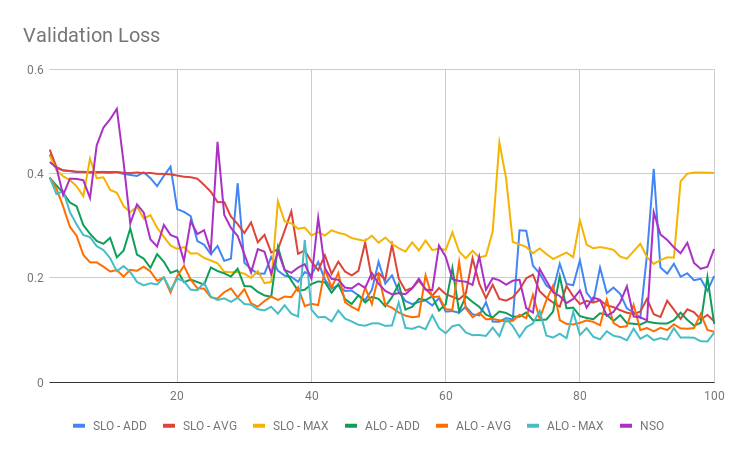
\includegraphics[width=1.\columnwidth]{figures/falreis/validation_loss.png}
  \label{fig:validation_loss}
\end{figure}

From previous graph, it is possible to conclude that ALO networks had superior and more desirable behavior than the SLO and NSO models. It is believed that these results are consequence of the considerably larger amount of side-outputs, which create more possibilities of interchangeability between confident values.

\subsection{Best results}

In order to improve the results, a new set of tests were performed using 500 training epochs. As some networks had a poor performance in the previous test and other tests with different parameters, we decided to evaluate all ALO networks in this new round of tests. For comparison, we also trained NSO network.

To measure the performance in our tests we use two different metrics. The first one is the well known categorical cross entropy accuracy. Also, we use an metric called pixel-error. This measure evaluates the number of pixels incorrectly classified over the total number of the pixels (number of wrong pixels). The metric was adopted when we observed high values of accuracy in results in which there were visibly many errors, mainly in the existence of numerous false positives. These two metrics are available in Figure \ref{fig:val_acc_500_epochs}.

\begin{figure*}
  \caption{Categorical Cross Entropy Validation Accuracy and Pixel-Error results for 500 epochs test set}
  \centering
  \begin{tabular}{ll}
    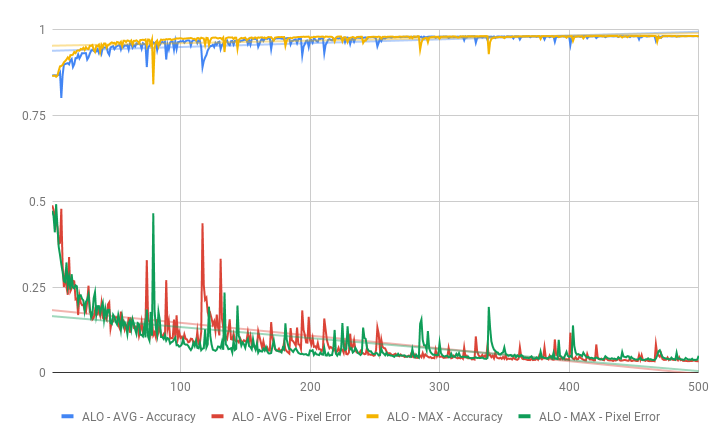
\includegraphics[width=1.\columnwidth]{figures/falreis/val_acc_500_epochs.png}
  
    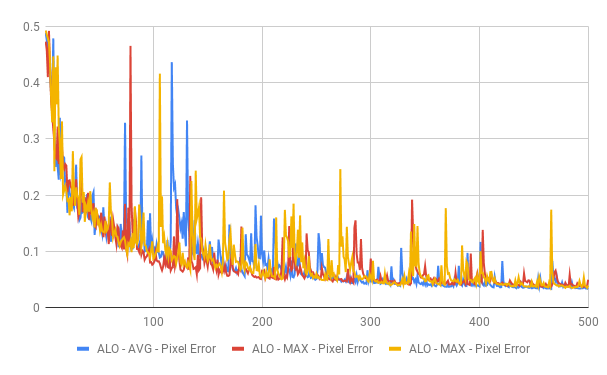
\includegraphics[width=1.\columnwidth]{figures/falreis/pixel_error_500_epochs.png}
  \end{tabular}%
  \label{fig:val_acc_500_epochs}
\end{figure*}

Is clearly visible in Figure \ref{fig:val_acc_500_epochs} that side-outputs influences the performance of the networks. All ALO networks had overall performance better than NSO network. Also, the learning curve of ALO networks shows that the network learns faster when use multiple side outputs. At last, it is possible to use bigger learning rate parameters, increasing the learn in early times.

The best results of both metrics are quite similar for all networks. This indicates absence of a far better ALO method to combine side-outputs. The best result for cross entropy validation metric is just \textbf{0.0009} above the worst one (0.983 for ALO-ADD and 0.9821 for ALO-AVG). For pixel-error, the best value is just \textbf{0.0040} above the worst one (0.0332 for ALO-AVG and 0.0372 for ALO-MAX).

Due to the similarity of the results, we will indicate the best method using the value of validation pixel-error metric. Also, AVG fusion method was also previous used in \cite{xie2015} and \cite{liu2017} to combine the results. For this criteria, ALO-AVG was defined as the best method of our training set.

\subsection{Post-processing using mathematical morphology}

%\remEwai{Insert reference to section IV that describes that post-processing. \cite{najman13} should go in section IV.} \remFeli{Partial Done}

After the training procedure, we create a post processing step to reduce possible noises in results proposition. For this, we used the mathematical morphology operation of Opening, as defined in Section \ref{ssec:post_processing}. This procedure removes small noises created by the foreground~(the road) in the background. 

The opening operation was applied using square structuring elements full of ones. We decided to use a set of kernels with sizes of $5\times5$, $7\times7$, $9\times9$, $11\times11$ and $13\times13$, sequentially applied into the image. This type of operation, although unusual, achieved the best results. It allowed that sections incorrectly classified by the network could be eliminated by the sequential thinning of noises in different shapes. The results also become more smooth with this procedure.

%\remEwai{I don't understand here. All the structuring elements are applied sequentially? which makes no sense since the opening by the largest structuring element is included in the opening by the smallest structuring element if I'm right. Or are they all tested independently? In this latter case, which size is finally retained?} \remFeli{Yes, sequencially. Although unusual, it removed incorrect classification better than small kernels alones. (Text changed for better explanation)}

A simple comparison of our procedure with the original network prediction is presented in Figure \ref{fig:post_processing_comp}. In this image, we selected an output result that clearly shows the benefits of mathematical morphology post processing. It is possible to see the removal of part of the noise in the far right of the image (\textit{white pixels}). The noise removal increases the confidence, as small variations in the results can lead to a potential problem, if used in a self-driving vehicle. 

\begin{figure}
  \caption{Comparison between ALO-AVG without post processing and ALO-AVG with post-processing with mathematical morphology. In the last picture, \textit{white} pixels represents desirable differences while \textit{red} pixels represents undesirable ones.}
  \centering
  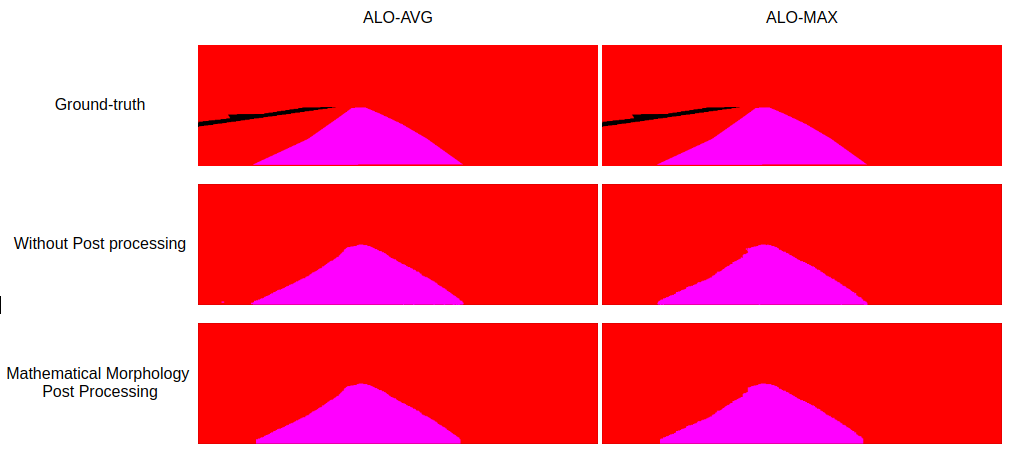
\includegraphics[width=1.\columnwidth]{figures/falreis/post_processing_comparison.png}
  \label{fig:post_processing_comp}
\end{figure}

A side effect of this method is the removal of some points that seems to fit correctly. This situation happens frequently in the base of the road proposition. In Figure \ref{fig:post_processing_comp}, it can be seen in the bottom left and the bottom right of the road (\textit{red pixels}).

\subsection{Side-outputs contribution in each merging strategy}
\label{ssec:merging_learn}

Each layer of each merging strategies learns in its particular way. The merging strategy influences how the networks learn. It is possible to see how each side-output learns and contributes to the final output in Figure \ref{fig:side_outputs}. To simplify the study of side-outputs, we decided to visualize only the last  output from each stage in \textbf{ALO} network, for our trained networks. To make the layers outputs easier to analyse, the images were  converted to black and white, where white pixels were classified as road and black pixels were classified as background.

%\remEwai{Not clear relatively to Fig. 2} \remFeli{Changed section. Removed Fig. 2 information.}

\begin{figure*}
  \caption{Side outputs for each merging strategy in ALO network.}
  \centering
  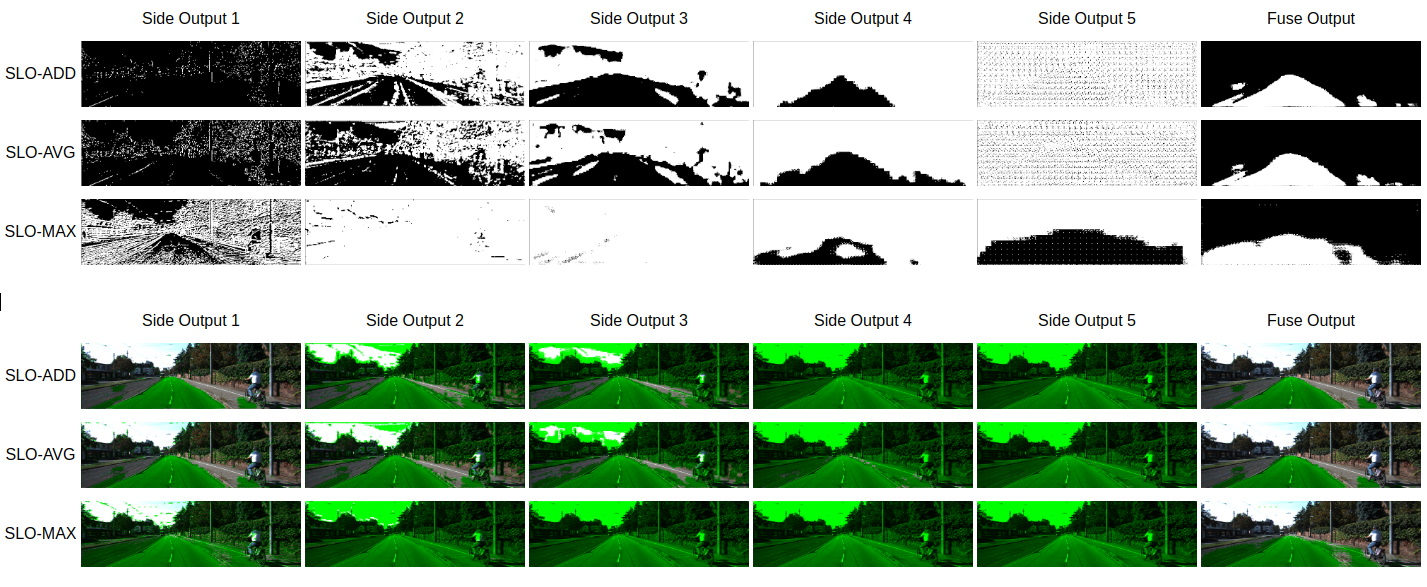
\includegraphics[width=1.0\textwidth]{figures/falreis/side_outputs.png}
  \label{fig:side_outputs}
\end{figure*}

%\remEwai{Fig. \ref{fig:side_outputs} is not so clear. Notation from the text should be reused: the side-output i what is denoted $\mathcal{H}_i$ (if I'm correctly understanding)} \remFeli{Changed. I don't know if it was clear enough. I'll think in how to improve it}

Figure \ref{fig:side_outputs} indicates that the first two stage side-outputs (outputs $\mathcal{H}_2$ and $\mathcal{H}_4$) does not produce significant information. Images are almost white, indicating that all pixels were classified as road. ALO-AVG and ALO-ADD third layer contains a clear separation between road pixel than non-road pixels. ALO-MAX's third layer, on the other hand, does not clearly separate road from non-road pixels. The results are pixelated and blur when compared with the original image.

Figure \ref{fig:side_outputs} also indicates that fourth stage side-output layer (output $\mathcal{H}_{10}$) clearly contains the best side-output for all ALO networks. The road marks are clearly visible, but with some noise. ALO-MAX contains a lot of noise, while ALO-ADD contains a few ones. The final stage side-output ($\mathcal{H}_{13}$) contains a lot of noise, with results far away worse than the previous layer. This possibly indicates that the layer was not able to correctly learn the information from the previous ones.

The fuse layer combine all side-outputs (including the ones not shown in Figure \ref{fig:side_outputs}) in order to predict. Despite poor results on some layers, the learning process adjusts itself so that even very few accurate results can be used by the model, similar to ensemble methods.

%\remEwai{= the proposition $Z$} \remEwai{? Not clear} \remEwai{merging layers = fuse layer?} \remFeli{Fixed. Text improved but I don't know if it is good enough. I don't know if I can cite ensemble methods.}

\subsection{Evaluation results and comparison with the state-of-the-art}

Reminding that the test evaluation could only be performed using KITTI Server, the metrics provided are maximum F1-measure~(MaxF), average precision~(AP), precision~(PRE), recall~(REC), false positive rate~(FPR) and false negative rate~(FNR). 

The server tests were performed using ALO-AVG method, the best one in the training process. To provide succint labels, we will use the name \textbf{ALO-AVG-MM} for our version with mathematical morphology post-processing. The results achieved  on the test set according to each category in the road scenes are presented in Table~\ref{tab:metrics}. 

\begin{comment}
{\color{As expected, the ALO-AVG-MM model performs better then the ALO-AVG in almost all the cases. red}It is also possible to notice that although the post-processing slightly improves the overall performance, it also increases the number of false negatives. This could be an indication that perhaps the applied kernel sizes are not adequate and are removing more of the foreground than desired.}
\end{comment}

If compared with the best result in KITTI Server platform~(called \textit{PLARD}, an anonymous submission\footnote{Results accessed in 2018-01-14. The method used was not described and no paper publishing information was provided.}), the results had overall performance 5.0\% below. Compared with the best paper submission \cite{Caltagirone2018}, the results were 4.0\% below. Once our model was trained only for 500 epochs with high learning rate, it is expected to achieve better results with fine tunning of our model, which is not the main focus of this paper. Also, it is important to notice that we didn't used methods to increase precision like bird-eye-view transformations and space color changes, that can improve the precision of the model.

\begin{table}
 \scriptsize
 \caption{KITTI benchmark evaluation results for each category}
  \begin{tabular}{{l}{c}{c}{c}{c}{c}{c}}
  
   \multicolumn{7}{l}{\textbf{um\_road}} \\
  \hline 
    Method & MaxF & AP & PRE & REC & FPR & FNR \\
  \hline
    \textit{SLO} & 96.92\% & 87.36\% & 94.47\% & \textbf{99.49\%} & 1.13\% & \textbf{0.51\%} \\
    \textit{SLO-mm} & \textbf{97.01}\% & \textbf{87.68\%} & \textbf{94.83\%} & 99.30\% & \textbf{1.05\%} & 0.70\% \\
    \textit{ALO}  & 96.39\% & 86.81\% & 93.87\% & 99.05\% & 1.25\% & 0.95\% \\
    \textit{ALO-mm} & 96.65\% & 87.51\% & 94.64\% & 98.74\% & 1.08\% & 1.26\% \\
    \textit{State-of-the-art} & \textbf{97.05\%}& \textbf{93.53\%} &\textbf{97.18\%} &\textbf{96.92\%} &	\textbf{1.28\%} &\textbf{3.08\%} \\
  \hline
  \multicolumn{7}{c}{} \\
  
  \multicolumn{7}{l}{\textbf{umm\_road}} \\
  \hline 
    Method & MaxF & AP & PRE & REC & FPR & FNR \\
  \hline
    \textit{SLO}  & 97.57\% & 89.44\% & 96.05\% & \textbf{99.15\%} & 1.24\% & \textbf{0.85\%} \\
    \textit{SLO-mm} & \textbf{97.61\%} & \textbf{89.67\%} & \textbf{96.30\%} & 98.97\% & \textbf{1.16\%} & 1.03\% \\
    \textit{ALO}  & 97.05\% & 88.83\% & 95.37\% & 98.78\% & 1.46\% & 1.22\% \\
    \textit{ALO-mm} & 97.21\% & 89.31\% & 95.90\% & 98.56\% & 1.29\% & 1.44\% \\
    \textit{State-of-the-art} & \textbf{97.77}\%&\textbf{ 95.64\%} &\textbf{97.75\%} &\textbf{97.79\%} &	\textbf{2.48\%} &\textbf{2.21\%} \\
  \hline
  \multicolumn{7}{c}{} \\
  
  \multicolumn{7}{l}{\textbf{uu\_road}} \\
  \hline 
    Method & MaxF & AP & PRE & REC & FPR & FNR \\
  \hline
    \textit{SLO}   & 95.16\% & \textbf{85.73\%} & 92.94\% & 97.49\% & 1.16\% & 2.51\% \\
    \textit{SLO-mm}  & \textbf{95.42\%} & 86.48\% & \textbf{93.77\%} & 97.13\% & \textbf{1.01\%} & 2.87\% \\
    \textit{ALO}   & 94.70\% & 84.87\% & 92.00\% & \textbf{97.56\%} & 1.33\% & \textbf{2.44\%} \\
    \textit{ALO-mm} & 95.20\% & 86.15\% & 93.40\% & 97.08\% & 1.08\% & 2.92\% \\
    \textit{State-of-the-art} & \textbf{95.95\%}& \textbf{95.25\%} &9\textbf{5.25\%} &\textbf{95.65\%} &	\textbf{1.21\%} &\textbf{4.35\%} \\
  \hline
  \multicolumn{7}{c}{} \\
  \end{tabular} 
  \label{tab:metrics}
\end{table}


To show the performance of our model, a visual representation of ALO-AVG-MM predictions are presented in Figure \ref{fig:visual_representation}. This image shows the true positives predictions marked in green, false negatives marked in  red and false positives marked in blue. The image contains results provided by Kitti Evaluation Server, based in the generated binary map sent to the server.

\begin{figure}
  \caption{Visual representation of the results. The generated image was provided by Kitti Evaluation Server. Green pixels represents true positives, red pixels are false negatives and blue pixels are false positives.}
  \centering
  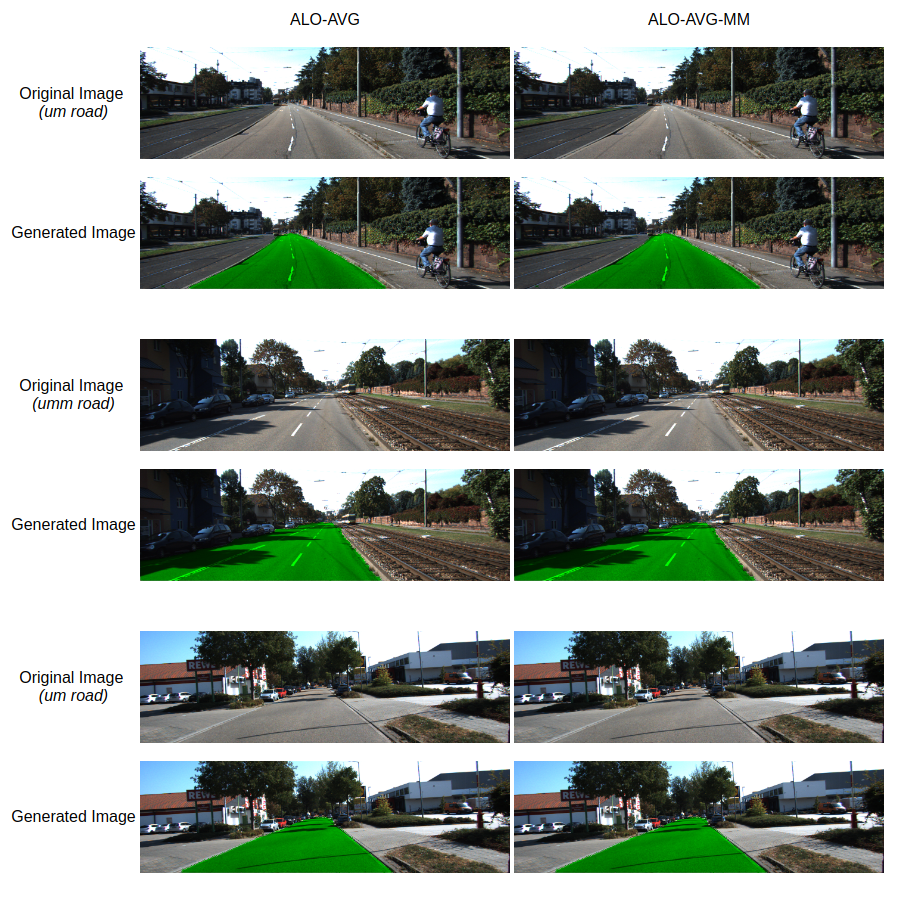
\includegraphics[width=1.\columnwidth]{figures/falreis/visual_representation.png}
  \label{fig:visual_representation}
\end{figure}

\section{Conclusion}
\label{sec:conclusion}

This work addressed the problem of merging side-outputs extracted from the convolutional layer model VGG to create region propositions for the task of image segmentation. We compare 3 different merging strategies to combine the side results: $add()$, $avg()$ and $max()$. The functions to enhance were evaluated using a cross-entropy and pixel-error loss functions. The impact of the number of side-outputs was studied and compared to a version without any side-outputs for a similar network architecture. At last, a simple mathematical morphology operation was proposed to  enhance the performance on the task and remove some noises. 

Experiments demonstrated that the $avg()$ function is viable for merging maps with different sizes and connotations, and could place the proposed strategy among the state-of-the-art approaches for the task on the Kitti dataset. The use of $avg()$ merging strategy was adopted before in \cite{liu2017}, but no explanation was given to the use of this method over other possible merging strategies. This paper helps to explain the good results achieved by those researchers.

It was also demonstrated that a large amount of side-outputs increases the network capabilities during the training step and could also creates jumps that could lead to better performance, in terms of accuracy. The training graphs also shows that the number of side-outputs contributes to a faster decay in loss function and stable results. The post-processing strategy slightly improved the performance, but requires further studies.

This research opens novel opportunities for study such as: (i) exploring different merging functions, less susceptible a values fluctuations;  (ii) exploring regularization techniques to sustain larger amounts of side-outputs consistent; and (iii) insert the mathematical morphology kernels on the learning process to search for the best kernel size. 
 
The code  and a file containing all dependencies to reproduce the experiments is public available online in \url{https://github.com/falreis/segmentation-eval}. 

\section{Acknowledgements}
\label{sec:acknowledgements}

This paper acknowledges Github repositories \url{https://github.com/lc82111/Keras_HED} and \url{https://github.com/moabitcoin/holy-edge} that were helpful to provide some basic source codes used in this work.




\bibliographystyle{IEEEtran}
\bibliography{2019-ijcnn,dl}

\end{document}
